\chapter{Introduction on quantum computing}

Introduction on quantum computing
In this chapter, I will present some basic concepts of quantum computing, and they will be useful for the following chapters, where I will instead discuss the process for correcting quantum errors. In the first section, I will discuss the fundamental unit of quantum information: the Qubit. The second section deals with how we can manipulate qubits through quantum logic gates. The third section instead discusses the density matrix, which is a useful tool for representing mixed states. In the end, the fourth section is a description of what noise and decoherence of a state are. Last but not least, the concept of fidelity is presented, a measure that indicates how similar the two states are.


\section{Qubits}
Classical computers and classical information rely on the concept of bit. The bit is the fundamental unit of classical information, i.e. the smallest portion into which any encoded information can be broken down; it is, therefore, the unit of measurement of encoded classical information.

Just as the bit is the smallest amount of information in classical computation, quantum computation is based on an analogous concept: the quantum bit or qubit.

A classical bit's state can be either 0 or 1, it can be turned off or turned on. The difference between bits and qubits is that a qubit can be in a state other than $|0\rangle$ or $|1\rangle$ (we use the bracket notation to identify the computational basis).
Indeed, if we are dealing with qubits it is also possible to form linear combinations of states, often called superpositions:
$$
|\psi\rangle=\alpha|0\rangle+\beta|1\rangle .
$$
The numbers $\alpha$ and $\beta$ are complex numbers and are called amplitudes.
However, when we measure a qubit we get either the result 0, with probability $|\alpha|^{2}$, or the result 1, with probability $|\beta|^{2}$. Naturally, $|\alpha|^{2}+|\beta|^{2}=1$, since the probabilities of all the possible outcomes must sum to one. 

In other words, a qubit can be represented by a vector in the two-dimensional complex Hilbert space $\mathbb{C}^2$, where $\ket{0}$ and $\ket{1}$ are known as computational basis states and form an orthonormal basis for this vector space.
Up to a global (and unphysical) phase factor, any single qubit can be expressed as follow: 
$$
|\psi\rangle=\cos \frac{\theta}{2}|0\rangle+e^{i \varphi} \sin \frac{\theta}{2}|1\rangle ,
$$
where $\theta, \varphi$ are real numbers. 
The numbers $\theta$ and $\varphi$ define a point on the unit three-dimensional sphere, as shown in \ref{sphere:bloch}.

\begin{figure}[h!]
    \centering
    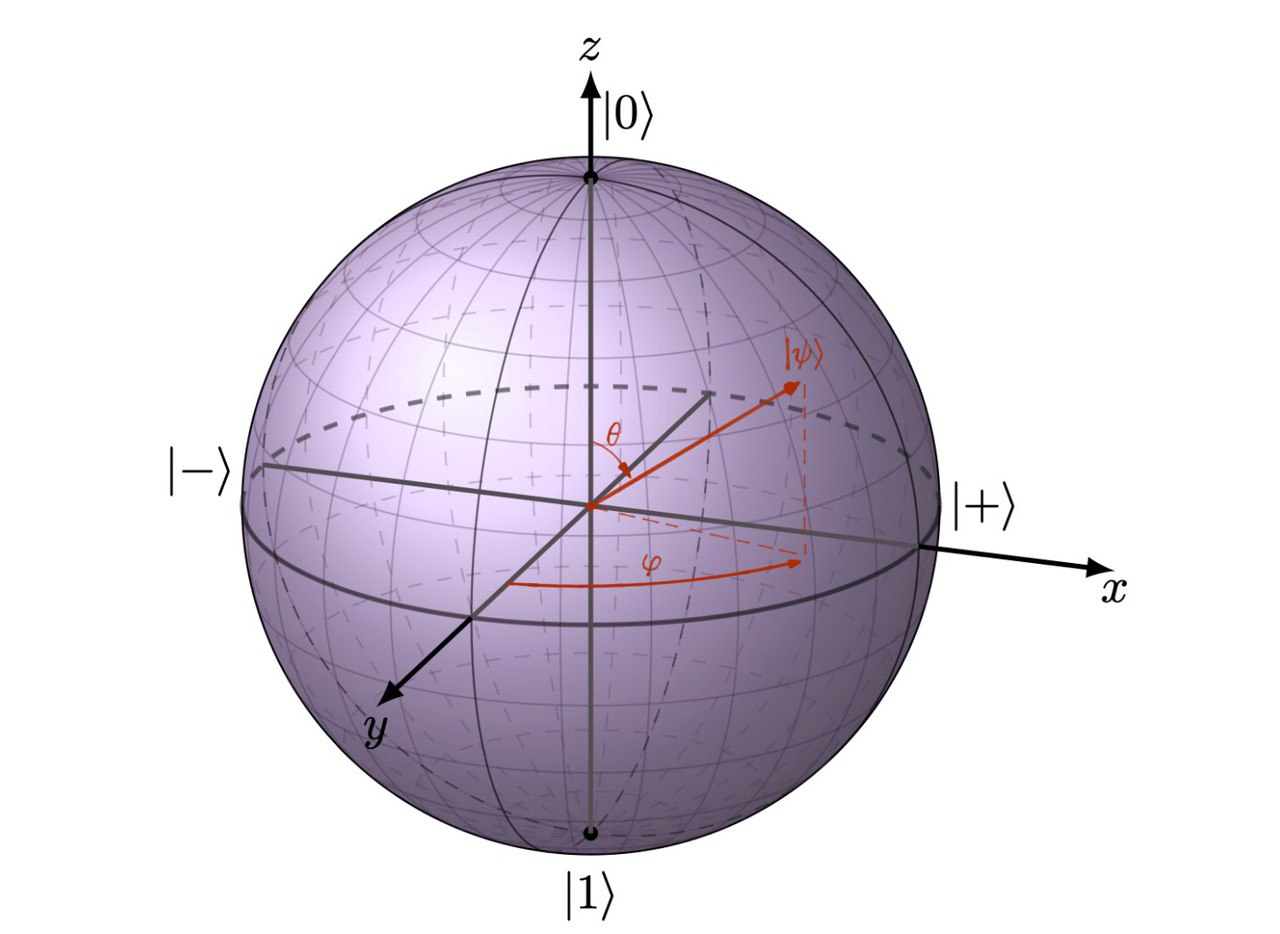
\includegraphics[scale=0.25]{Mainmatter/images/blochhh.jpg}
    \caption{Bloch sphere}
    \label{sphere:bloch}
\end{figure}
This sphere is called the Bloch sphere and provides a useful means of visualizing the state of a single qubit, and often serves as an excellent test for ideas about quantum computation and quantum information.
Many of the operations can be done on a single qubit, through logic gates, and they can be described within the Bloch sphere picture.
However, it must be kept in mind that this intuition is limited because there is no simple generalization of the Bloch sphere known for multiple qubits.

A system of multiple qubits is represented by tensor-product Hilbert spaces; for example, a system composed of two qubits has a state
$|\psi\rangle$ belonging to the tensor product of the Hilbert spaces of the two individual qubits, and we say that $|\psi\rangle \in \mathcal{H}_1 \otimes \mathcal{H}_2$. However, in this and in even larger spaces, there is a fundamental and physically crucial difference between the two kinds of states. There are the so called factorizable states, which can be expressed in the form of tensor product: 
\begin{equation*}
    \ket{\psi} = \left(\alpha_{1}|0\rangle_{1}+\beta_{1}|1\rangle_{1}\right) \otimes[\ldots] \otimes\left(\alpha_{n}|0\rangle_{n}+\beta_{n}|1\rangle_{n}\right)
\end{equation*}
and there are also the  entangled states which are "un-factorizable", i.e the quantum state cannot be factorised as a product of states of its local constituents. 
A perfect example can be provided by considering a two qubits system; a factorizable state is: 
$$
\left|\psi_{f}\right\rangle=(\alpha_1\alpha_2|00\rangle+\alpha_1\beta_2|01\rangle+\beta_1\alpha_2|10\rangle+\beta_1\beta_2|11\rangle)=(\alpha_1|0\rangle+\beta_1|1\rangle) \otimes(\alpha_2|0\rangle+\beta_2|1\rangle)
$$
while an example of entangled state could be:
$$
\left|\psi_{e}\right\rangle=\alpha|00\rangle+\beta|11\rangle.
$$


%A state system of multiple qubits can be expressed as the n-fold tensor product between all the Hilbert space of the single qubit. For example, a system of n qubits lies in $\mathcal{H}=\mathcal{H}_1 \otimes \mathcal{H}_2 \otimes\mathcal{H}_3 \otimes ... \otimes\mathcal{H}_{n-1} \otimes\mathcal{H}_n$.


%The concepts relating to quantum computation and, in particular, the concept of qubits are based on quantum mechanics.
%The physical layer is therefore endowed with properties that cannot be observed in the macroscopic world, such as superposition of states, interference, entanglement and indeterminacy.
Qubit states can be manipulated and transformed in ways that lead to measurement outcomes that depend distinctly on the different properties of the state. 
However, in the end, we cannot measure a qubit in its state of superposition but we can manipulate the amplitudes to get the result which we are looking for.
A quantum computer can create vast multidimensional spaces in which to represent very large problems, solve the problem using the properties of quantum mechanics, some logic gates, and operations. One of the techniques consists in adjusting the amplitude contributions, in fact, if some amplitudes are positive and others are negative, then the contributions can interfere destructively and cancel each other out. %so that the amplitude is zero and the corresponding outcome is never observed;
Likewise, they can interfere constructively and increase the likelihood of a given outcome. The goal in devising an algorithm for a quantum computer is to choreograph a pattern of constructive and destructive interference so that for each wrong answer the contributions to its amplitude cancel each other out, whereas for the right answer the contributions reinforce each other. If you can arrange that, one will see the right answer with a large probability when one measures. The tricky part is to do this without knowing the answer in advance, and faster than you could do it with a classical computer.



Another important question is: how much information can be carried by a qubit?
Paradoxically, a qubit can exist in a continuum of states between the two bases, so there are an infinite number of linear combinations of the orthonormal basis apparently allowing, at least in principle, the representation of all human knowledge in a single qubit.

However, this is an erroneous conclusion by virtue of the behavior of the qubit during measurement. It must be kept in mind, in fact, that the outcome of the measurement of the state of a qubit can only be $\ket{0}$ or $\ket{1}$, with respective probabilities $|\alpha|^2$ and $|\beta|^2$. We can interpret this as the condition that the qubit’s state is normalized to length $1$. 
Moreover, the measurement of the qubit inexorably changes its state, collapsing the superposition state in one of the two specific states represented by the vectors of the computational basis as prescribed by the postulate of measure in quantum mechanics.

Thus, from the measurement of a qubit, it is possible to obtain the same amount of information that can be represented by a classical bit. This result has been proved rigorously by Holevo's Theorem.








There is currently no preferred qubit technology, a variety of physical systems are being explored for use as qubits: the two different polarizations of a photon, as the alignment of a nuclear spin in a uniform magnetic field... 
In contrast, bits in a classical computer are typically realized as the robust on/off states of transistor switches which are differentiated by billions of electrons.
A shortcoming shared by all of these approaches to realize a quantum computer is that it is difficult to sufficiently isolate the qubits from the effects of external noise, meaning errors during quantum computation are inevitable, and quantum error correction codes have been developed in order to protect a qubit from the external noise. After this introduction in \ref{chap:2} I will describe how these codes work. 


\section{Quantum gates}\label{sec:qgate}

Classically one can manipulate a system of bits and make some operations on it, using logic gates in order to solve a certain problem. Analogous to the way a classical computer is built from an electrical circuit containing wires and logic gates, a quantum computer is built from a quantum circuit containing wires and elementary quantum gates to carry around and manipulate the quantum information.
A quantum gate can be represented as an operator acting on the states of one or more qubits, depending on the nature of the gate.
A qubit can be represented as a two-dimensional ket. Thus, the operator algebra acting on those kets is 4-dimensional. 


A quantum gate has to preserve the normalization condition of a state $|\psi\rangle$. Given an operator $\hat{U}$ that transforms $|\psi\rangle \rightarrow\left|\psi^{\prime}\right\rangle$, it follows:
$$
\left\langle\psi^{\prime} \mid \psi^{\prime}\right\rangle =\bra{\psi}\hat{U}^{\dagger} \hat{U}\ket{\psi}=1
$$
Hence, 
$$
 \hat{U}^{\dagger} \hat{U}=\widehat{\mathbb{I}}
$$
Operators satisfying this condition are called unitary operators. This imply that all quantum gates are also reversible, in fact, equation  prove that $\hat{U^{-1}}$ exists and it is equal to $\hat{U}^{\dagger}$, thus:
$$
\hat{U}^{\dagger}\left|\psi^{\prime}\right\rangle=\hat{U}^{\dagger} \hat{U}|\psi\rangle=\hat{\mathbb{I}}|\psi\rangle=|\psi\rangle
$$
If we consider a one qubit system, a suitable basis for these unitary operators acting on the system can be given by the identity matrix and the pauli matrices: 
$$
I=\left(\begin{array}{cc}
1 & 0 \\
0 & 1
\end{array}\right) \quad  \sigma_X=X=\left(\begin{array}{cc}
0 & 1 \\
1 & 0
\end{array}\right) \quad 
\sigma_Y=Y=\left(\begin{array}{cc}
0 & -i \\
i & 0
\end{array}\right) \quad
\sigma_Z=Z=\left(\begin{array}{cc}
1 & 0 \\
0 & -1
\end{array}\right).
$$
All these matrices are unitary and also hermitian, which implies that $\sigma_i=\sigma_i^{-1} \quad \forall i = X,Y,Z$, where $\sigma$ represent one of the 3 pauli matrices. Moreover, the Pauli matrices satisfy the following relations:
$$
\begin{aligned}
\sigma_{i} \sigma_{j} &=\delta_{i j} \mathbb{I}+i \epsilon_{i j k} \sigma_{k} \\
\left[\sigma_{i}, \sigma_{j}\right] &=2 i \epsilon_{i j k} \sigma_{k} \\
\left\{\sigma_{i}, \sigma_{j}\right\} &=2 \delta_{i j} \mathbb{I}
\end{aligned}
$$
where $\epsilon_{i j k}$ is the Levi-Civita symbol, $[\cdot, \cdot]$ is the commutator and $\{\cdot, \cdot\}$ is the
anticommutator.
These 4 matrices provide a basis of the operators acting on a single qubit. It follows that every single qubit operator can be expressed as a linear combination of $I,X,Y,Z$: 
\begin{equation*}
    U = \alpha I+\beta X+\gamma Y+\delta Z \quad \text{with $\alpha,\beta,\gamma,\delta$ complex numbers}.
\end{equation*}
and a multi-qubit operator can be expressed as a tensor product of single qubit operators:
\begin{equation*}
    U = U_1 \otimes U_2 \otimes ... \otimes U_n.
\end{equation*}
Quantum gates are reversible by definition. Thus, the numbers of qubits in input must be the same as the qubits in output, otherwise, the gates are not reversible. An immediate consequence of this property is, for instance, that the classical AND gate, largely used in classical computing, could not have an exact quantum analog.
Among all the quantum gates having as an input a single qubit, the most remarkable for our purpose are the quantum NOT, the Z gate, the Hadamard gate, and the general phase shift gate.
Instead, from all the gates that act on two qubits, the most important one in our context is the controlled-NOT gate.
In what follows we briefly introduce these gates. 

\subsection*{The quantum NOT gate}
In quantum circuits, it is represented by: \begin{figure}[H]
\centering
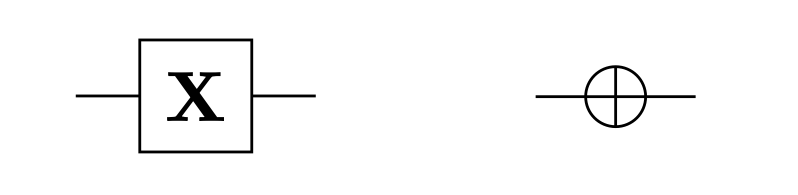
\includegraphics{Mainmatter/images/XGATE.png}
\end{figure}
Using the analogy with the classical NOT gate, which acts on the computational basis changing the state 0 in the state 1 and vice versa, one can suppose that the quantum not has the same action on the computational quantum basis, taking $\ket{0} \to \ket{1}$ and $\ket{1} \to \ket{0}$. It is interesting to see what happen to a state which is a superposition of the quantum basis: 
\begin{equation*}
    NOT \ket{\psi} = NOT(\alpha\ket{0} +\beta\ket{1}) = (\alpha\ket{1} +\beta\ket{0})
\end{equation*}
Thus, we can write down the "truth table", or better the action of the gate on the qubit: 
\begin{table}[h!]
    \centering
    \begin{tabular}{c|c}
         Input & Output \\
          $\ket{0}$ & $\ket{1}$ \\
          $\ket{1}$ & $\ket{0}$
    \end{tabular}
    \caption{Truth table quantum NOT gate}
    \label{tab:not_gate}
\end{table}


It is possible to notice that an operator which acts on a qubit like that is the X Pauli matrix, hence this gate it is also called X-gate.

\subsection*{The Z-gate}
In quantum circuits, this gate it is represented by \begin{figure}[H]
\centering
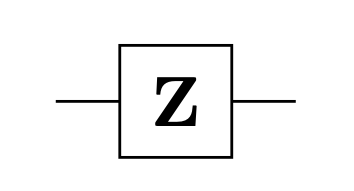
\includegraphics{Mainmatter/images/ZGATE.png}
\end{figure}.
This gate is represented by the Z pauli matrix. The associated "truth table" is: 
\begin{table}[h!]
    \centering
    \begin{tabular}{c|c}
         Input & Output \\
          $\ket{0}$ & $\ket{0}$ \\
          $\ket{1}$ & -$\ket{1}$
    \end{tabular}
    \caption{Caption}
    \label{tab:my_label}
\end{table}


This is a phase shifting in the space spanned by $\ket{0}$ and $\ket{1}$. However it can be understood as a bit-flip gate in other orthonormal basis states. For example, if we consider as computational basis $\ket{+}= \frac{\ket{0} + \ket{1}}{\sqrt{2}}$ and $\ket{-} = \frac{\ket{0} - \ket{1}}{\sqrt{2}}$, with respect to this new base elements, the action of the Z-gate is:
\begin{table}[h!]
    \centering
    \begin{tabular}{c|c}
         Input & Output \\
          $\ket{-}$ & $\ket{+}$ \\
          $\ket{+}$ & $\ket{-}$
    \end{tabular}
    \caption{"Truth table" of Z-gate in the new basis}
    \label{tab:not_gate}
\end{table}



Another interesting observation that can be seen is the action of the X-gate on a generic state $\ket{\psi} = \alpha \ket{+} + \beta \ket{-}$ in this new basis. In this new base the X matrix is: 
\begin{equation*}
    X_{\ket{+},\ket{-}} = M^{-1}X M = \left(\begin{array}{cc}
1 & 0 \\
0 & -1
\end{array}\right)  
\end{equation*}
Hence, the action of X in the new basis is the same as that of operator Z in the old basis.


\subsection*{The general phase-shift gate}
The Z gate is a particular case of the phase rotation gate, which corresponds to a phase shift of $\pi$. In quantum circuits, this gate it is represented by :
\begin{figure}[H]
\centering
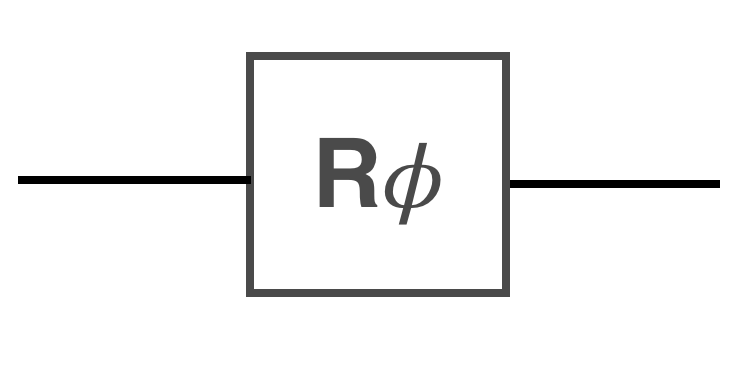
\includegraphics[scale=0.15]{Mainmatter/images/Phase_shift_gate.png}
\end{figure}
The phase-shift gate maps $\ket{0} \to \ket{0}$ and $\ket{1} \to e^{i\phi}\ket{1}$, where $\phi$ is the phase shift. It is possible to notice that if $\phi=\pi$. Thus, $e^{i\pi}=-1$ obtaining the Z-pauli matrix. The phase-shift $\phi$ can assume all the value from 0 to $2\pi$.

The probability of measuring a $\ket{0}$ or $\ket{1}$ is unchanged after applying this gate, however it modifies the phase of the quantum state.

The associated truth table is: 
\begin{table}[h!]
    \centering
    \begin{tabular}{c|c}
         Input & Output \\
          $\ket{0}$ & $\ket{0}$ \\
          $\ket{1}$ & $e^{i\phi}\ket{1}$
    \end{tabular}
    \caption{Truth table of R-gate}
    \label{tab:rotationgate}
\end{table}

The phase shift gate is represented by the matrix:
\begin{equation*}
     R_{\phi}=  \left(\begin{array}{cc}
1 & 0 \\
0 & e^{i\phi}
\end{array}\right)  .
\end{equation*}
But, sometimes in literature a different convention is adopted. In the following thesis I will specify always which one I use. 
To get an example of the other convention 
is usually represented with the $\theta$ angle.
\begin{equation*}
     R_{\theta / 2}=  \left(\begin{array}{cc}
1 & 0 \\
0 & e^{i\theta}
\end{array}\right)  .
\end{equation*}



\subsection*{The Hadamard gate}
In quantum circuits, this gate is represented by:
\begin{figure}[H]
\centering
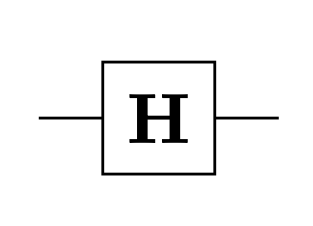
\includegraphics{Mainmatter/images/Hadamard_GAte.png}
\end{figure}
The hadamard gate acts on a single qubit creating a superposition if a basis state is given. It maps $\ket{0} \to \frac{\ket{0} + \ket{1}}{\sqrt{2}} = \ket{+}$  and  $\ket{1} \to \frac{\ket{0} - \ket{1}}{\sqrt{2}} = \ket{-}$. 
In particular, it corresponds exactly to the change of basis matrix from the $\{|0\rangle,|1\rangle\}$ to the $\{|+\rangle,|-\rangle\}$ bases and, thanks to the fact that it is self-reversible, also vice-versa. Its truth table is: 
\begin{table}[h!]
    \centering
    \begin{tabular}{cc}
\hline Input & Output \\
\hline$|0\rangle$ & $|+\rangle$ \\
$|1\rangle$ & $|-\rangle$ \\
\hline
\end{tabular}
    \caption{Caption}
    \label{tab:my_label}
\end{table}

And its matrix representation in the computational basis $\ket{0},\ket{1}$ is: 
\begin{equation*}
    H = \frac{1}{\sqrt{2}} \left(\begin{array}{cc}
1 & 1 \\
1 & -1
\end{array}\right)  
\end{equation*}

\subsection*{The controlled-NOT gate}
The CNOT gate acts on 2 qubits inverting the second qubit $\oplus$ (the target qubit) if and only if the first qubit $\Bigcdot$ (the control qubit ) is $\ket{1}$. In quantum circuit, it is represented by: 
\begin{figure}[H]
\centering
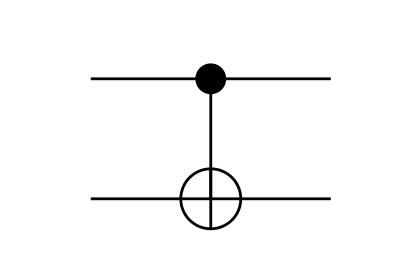
\includegraphics{Mainmatter/images/CNOT_gate.png}
\end{figure}
By being binary its truth table traces 4 different possible input scenarios: 
\begin{table}[h!]
    \centering
    \begin{tabular}{cc|cc}
    \hline
    \multicolumn{4}{c}{Input \quad \quad \quad \quad  \quad     Output } \\
    \hline Control& Target & Control & Target\\
\hline$|0\rangle$ & $\ket{0}$ & $\ket{0}$&$\ket{0}$\\
$|0\rangle$ & $|1\rangle$ &$|0\rangle$ & $|1\rangle$ \\
$|1\rangle$ & $\ket{0}$ & $\ket{1}$&$\ket{1}$ \\
$|1\rangle$ & $\ket{1}$ & $\ket{1}$&$\ket{0}$\\
\hline
\end{tabular}
    \caption{Action of the CNOT gate}
    \label{tab:my_label}
\end{table}
and so does the matrix representation which, this time, is based on a 4 × 4 matrix: 

\begin{equation*}
    CNOT =  \left(\begin{array}{cccc}
1 & 0 & 0 & 0\\
0 & 1 & 0 & 0\\
0 & 0 & 0 & 1\\
0 & 0 & 1 & 0\\
\end{array}\right)  
\end{equation*}
This gate is widely used to creates
entangled states. As an example, consider this circuit: 
\begin{figure}[h!]
    \centering
    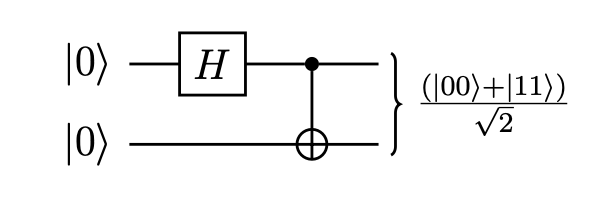
\includegraphics[scale=0.5]{Mainmatter/images/CNOT_entangled.png}
\end{figure}


where the final state is also known as $\ket{\Phi^+}$ Bell state.
Starting from the second chapter, we are going to use these gates to build quantum circuits for quantum error correction codes. Instead, in the last chapter I will focus more on how to make these gates more reliable. 